\documentclass{article}
\usepackage{amsmath}
\usepackage[utf8]{inputenc}
\usepackage{graphicx}
\usepackage{verbatim}
\usepackage{float}
\usepackage[makeroom]{cancel}
\usepackage[english]{babel}
\usepackage{textcomp}
\usepackage{gensymb}
\usepackage{color}
\usepackage{subcaption}
\usepackage{caption}
\usepackage{hyperref}
\usepackage{physics}
\usepackage{dsfont}
%\usepackage{amsfonts}
\usepackage{listings}
\usepackage{multicol}
\usepackage{units}

\usepackage{algorithmicx}
\usepackage{algorithm}% http://ctan.org/pkg/algorithms
\usepackage{algpseudocode}% http://ctan.org/pkg/algorithmicx

\usepackage[margin=1cm]{caption}
\usepackage[outer=1.2in,inner=1.2in]{geometry}
% For writing full-size pages
%\usepackage{geometry}
%\geometry{
%  left=5mm,
%  right=5mm,
%  top=5mm,
%  bottom=5mm,
%  heightrounded,
%}

% Finding overfull \hbox
\overfullrule=2cm

\lstset{language=IDL}
 %\lstset{alsolanguage=c++}
\lstset{basicstyle=\ttfamily\small}
 %\lstset{backgroundcolor=\color{white}}
\lstset{frame=single}
\lstset{stringstyle=\ttfamily}
\lstset{keywordstyle=\color{red}\bfseries}
\lstset{commentstyle=\itshape\color{blue}}
\lstset{showspaces=false}
\lstset{showstringspaces=false}
\lstset{showtabs=false}
\lstset{breaklines}
\lstset{aboveskip=20pt,belowskip=20pt}

\lstset{basicstyle=\footnotesize, basewidth=0.5em}
\lstdefinestyle{cl}{frame=none,basicstyle=\ttfamily\small}
\lstdefinestyle{pr}{frame=single,basicstyle=\ttfamily\small}
\lstdefinestyle{prt}{frame=none,basicstyle=\ttfamily\small}
% \lstinputlisting[language=Python]{filename}


\definecolor{codepurple}{rgb}{0.58,0,0.82}
\definecolor{backcolour}{rgb}{0.95,0.95,0.92}
\definecolor{dkgreen}{rgb}{0,0.6,0}
\definecolor{gray}{rgb}{0.5,0.5,0.5}
\definecolor{magenta}{rgb}{0.58,0,0.82}

\lstdefinestyle{pystyle}{
  language=Python,
  aboveskip=3mm,
  belowskip=3mm,
  columns=flexible,
  basicstyle={\small\ttfamily},
  backgroundcolor=\color{backcolour},
  commentstyle=\color{dkgreen},
  keywordstyle=\color{magenta},
  numberstyle=\tiny\color{gray},
  stringstyle=\color{codepurple},
  basicstyle=\footnotesize,
  breakatwhitespace=false,
  breaklines=true,
  captionpos=b,
  keepspaces=true,
  numbers=left,
  numbersep=5pt,
  showspaces=false,
  showstringspaces=false,
  showtabs=false,
  tabsize=2
}

%%%%%%%%%%%%%%%%%%%%%%%%%%%%%%%%
% Self made macros here yaaaaaay
\newcommand\answer[1]{\underline{\underline{#1}}}
\newcommand\pd[2]{\frac{\partial #1}{\partial #2}}
\newcommand\redrum[1]{\textcolor{red}{\textbf{#1}}}
\newcommand\numberthis{\addtocounter{equation}{1}\tag{\theequation}}
% Usage: \numberthis \label{name}
% Referencing: \eqref{name}

% Some matrices
\newcommand\smat[1]{\big(\begin{smallmatrix}#1\end{smallmatrix}\big)}
\newcommand\ppmat[1]{\begin{pmatrix}#1\end{pmatrix}}

% Title/name/date
\title{AST4310 - Stellar Spectra B}
\author{Simen Nyhus Bastnes\\simennb}
\date{11. November 2016}

\begin{document}
\maketitle
%\begin{abstract}
%wow dude, this is so abstract man
%\end{abstract}
\section*{Introduction}
In this exercise, we will study the formation of spectral lines in the solar atmosphere assuming Local Thermodynamical Equilibrium (LTE).
\section{Stratification of the solar atmosphere}
We study the radial stratification of the solar atmosphere on the basis of the standard model FALC.
\subsection{FALC temperature stratification}
\begin{figure}[H]
  \centering
  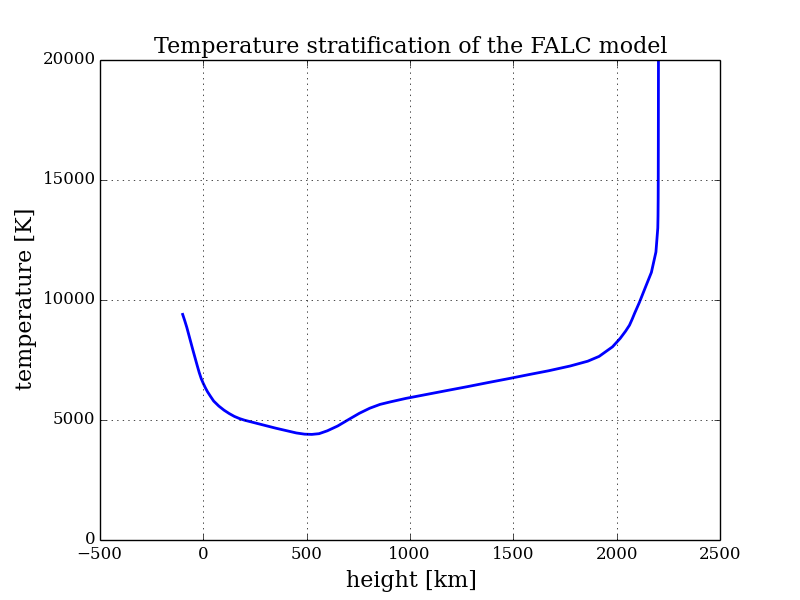
\includegraphics[scale=0.5]{../figures/falc/falc_h_temp.png}
  \caption{Temperature stratification of the FALC model. The height scale has $h=0$ at the location with $\tau_{500} = 1$. The photosphere reaches until $h=525$ km (temperature minimum). The chromosphere higher up has a mild temperature rise out to $h \approx 2100$ km, where it increases steeply as the corona starts.}
  \label{fig:falc_temp}
\end{figure}

\subsection{FALC density stratification}
\subsubsection{Total pressure against column mass}
\begin{figure}[H]
  \centering
  \begin{subfigure}{0.49\textwidth}
    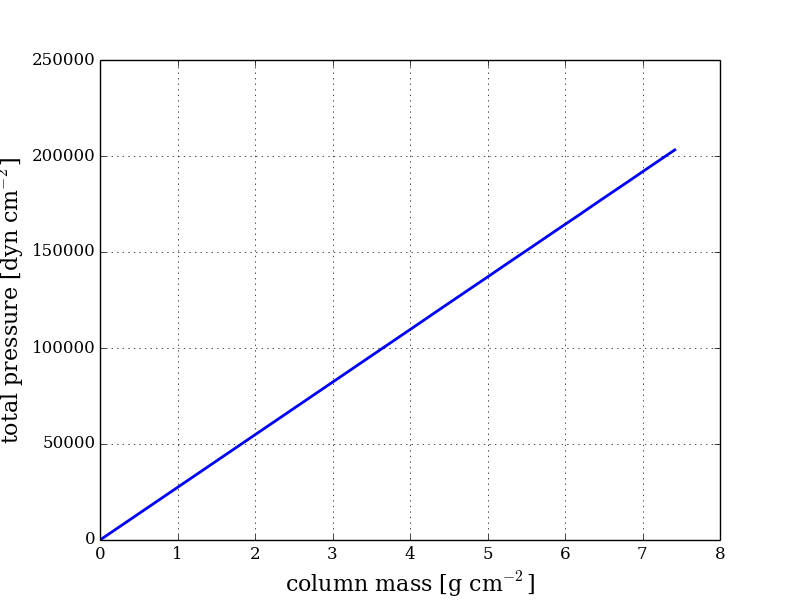
\includegraphics[scale=0.37]{../figures/falc/falc_colm_ptot.png}
    \caption{Total pressure against column mass, linearly scaled}
  \end{subfigure}
  \begin{subfigure}{0.49\textwidth}
    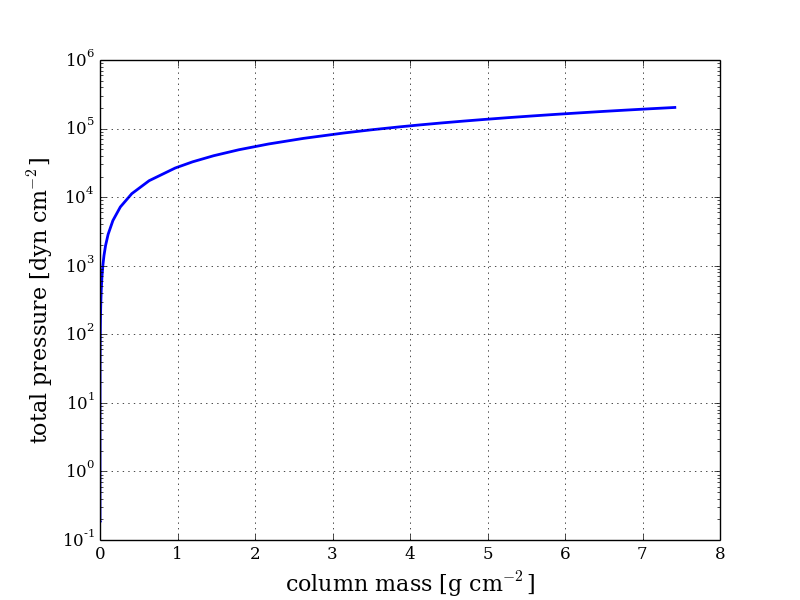
\includegraphics[scale=0.37]{../figures/falc/falc_colm_ptot_ylog.png}
    \caption{Total pressure against column mass, log. $y$-axis}
  \end{subfigure}
  \caption{In the panels in the figure, we have plotted the total pressure against the column mass, both linearly and with a logarithmic $y$-axis. As we see, the total pressure scales linearly. We can then write the relationship between pressure and column mass as $P = cm$, where $c$ is a constant with the units $[P/m] = [\text{cm}/\text{s}^2]$, which is acceleration. Since it is constant throughout the atmosphere of the sun, we can safely assume that it represents the gravitational acceleration at the surface of the Sun. We calculate this to be $c = g_{\text{surface}} = 27396.5$ cm/s$^2$}
\end{figure}

\subsubsection{Complete mixing}

\begin{figure}[H]
  \centering
  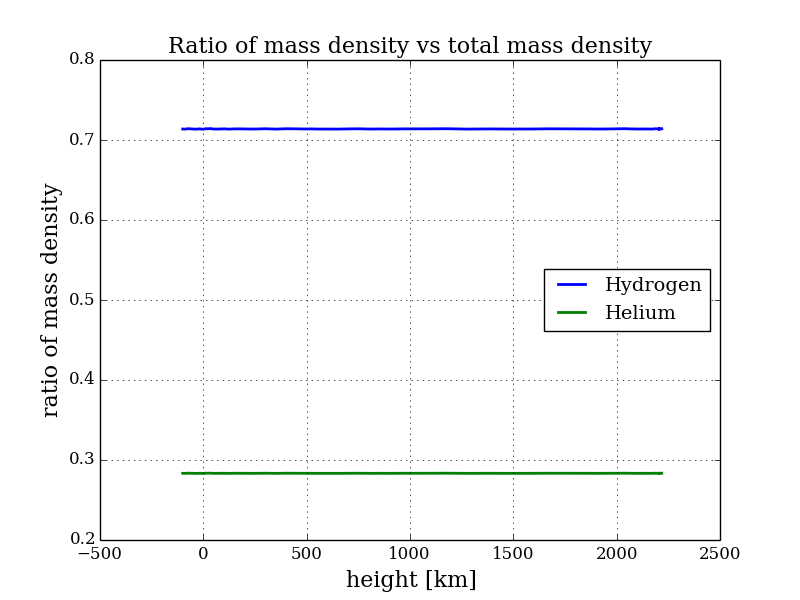
\includegraphics[scale=0.5]{../figures/falc/falc_h_dens.png}
  \caption{Plot of the relative abundance of hydrogen and helium. We see that the variations at different heights are very small for the elements, so the assumption of complete mixing holds up. The remaining fraction, we call metals, and calculate in our code that the fraction of metal is approximately $2.761\cdot10^{-3}$. We can then say that the sun consists of a bit over 70\% hydrogen, a bit less than 30\% helium, and $\approx0.3$\% metals.}
\end{figure}

\subsubsection{Column mass against height}
\begin{figure}[H]
  \centering
  \begin{subfigure}{0.49\textwidth}
    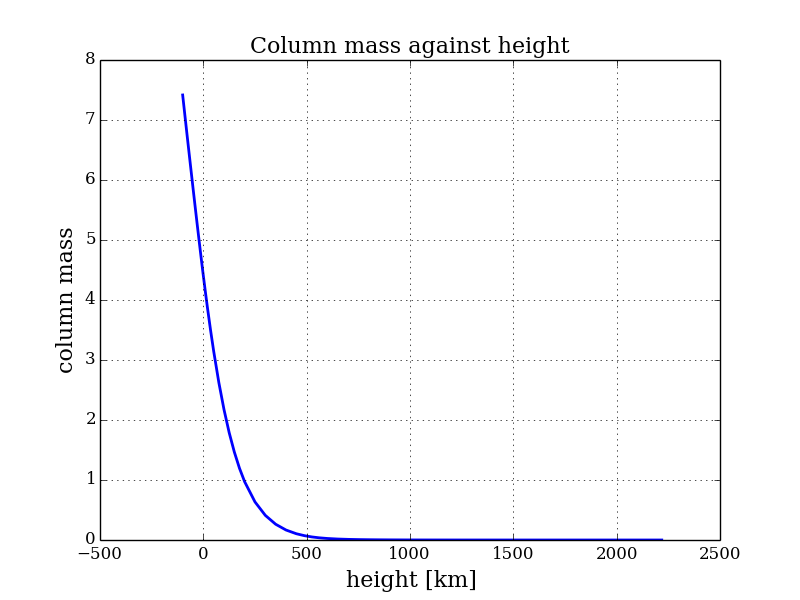
\includegraphics[scale=0.37]{../figures/falc/falc_h_colm_lin.png}
    \caption{Column mass against height, linearly scaled}
  \end{subfigure}
  \begin{subfigure}{0.49\textwidth}
    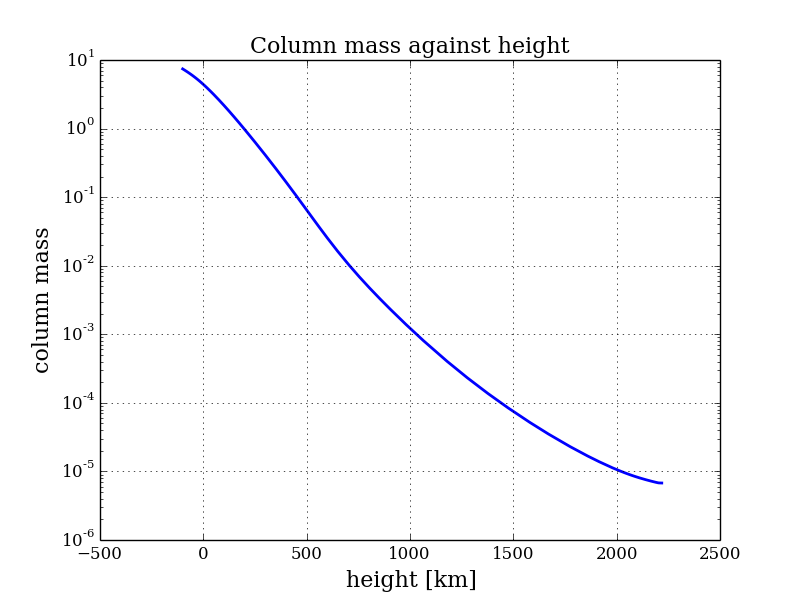
\includegraphics[scale=0.37]{../figures/falc/falc_h_colm_ylog.png}
    \caption{Column mass against height, log. $y$-axis}
  \end{subfigure}
  \caption{Column mass plotted against height for both linear and logarithmic $y$-axis. We observe that the column mass goes as $m\propto c^h$, since the mass density indreases towards the center of the Sun. From figure \ref{fig:falc_temp}, we know that the temperature does not increase logarithmically inwards, which affects the mass density, making the column mass not a fully straight line when plotted with logaritmic $y$-axis.}
\end{figure}

\subsubsection{Gas density against height}
\begin{figure}[H]
  \centering
  \begin{subfigure}{0.49\textwidth}
    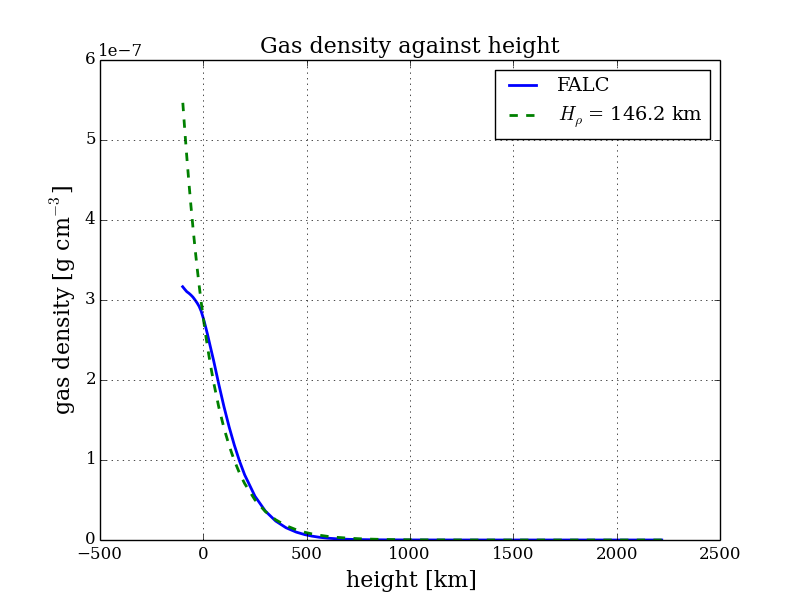
\includegraphics[scale=0.37]{../figures/falc/falc_h_dens2.png}
    \caption{Density against height, linearly scaled}
  \end{subfigure}
  \begin{subfigure}{0.49\textwidth}
    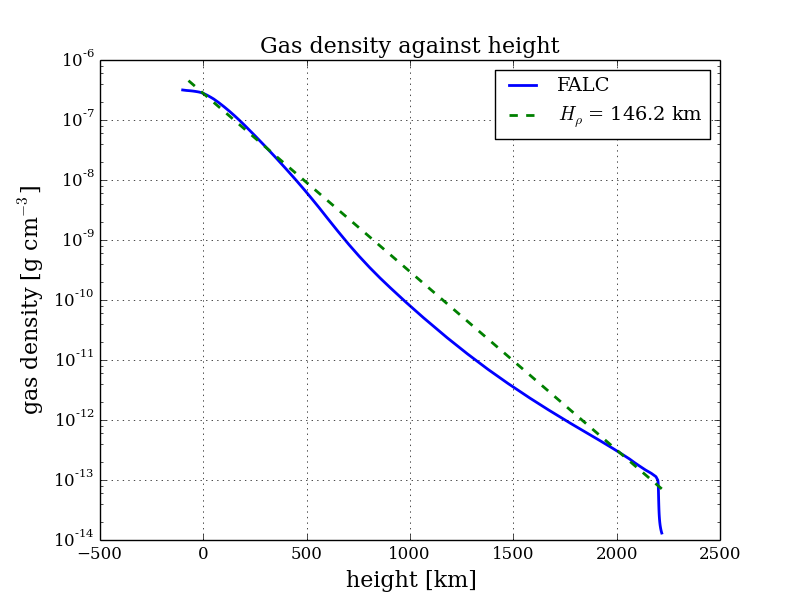
\includegraphics[scale=0.37]{../figures/falc/falc_h_dens3.png}
    \caption{Density against height, log. $y$-axis}
  \end{subfigure}

  \caption{Density against height in both linear and ylog plots. Overplotted in dashed lines is the density given by $\rho(0)\exp(-h/H_{\rho})$, with $H_{\rho}$ = 146.2 km in the deep photosphere.}
\end{figure}

\subsubsection{Gas pressure against height}
\begin{figure}[H]
  \centering
  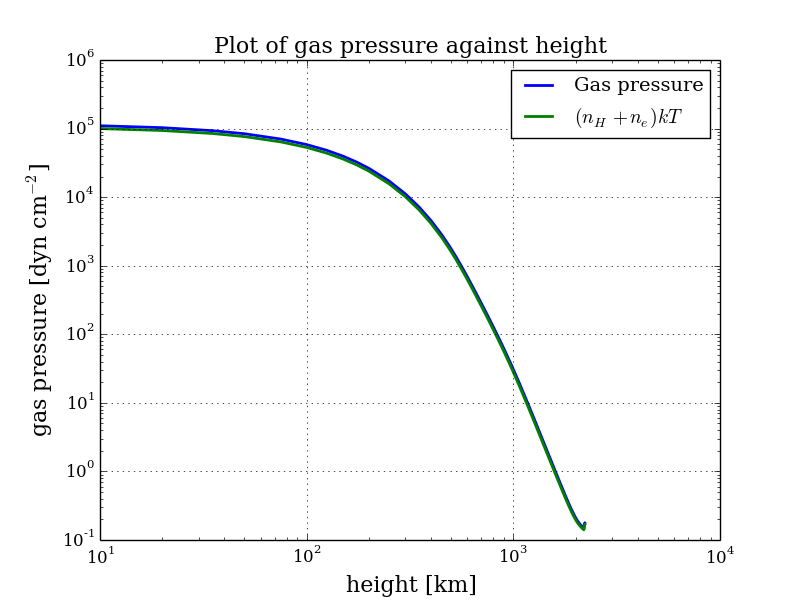
\includegraphics[scale=0.5]{../figures/falc/falc_h_pgas_0.png}
  \caption{Gas pressure from FALC plotted against height. Overplotted is the ideal gas law for a gas consisting only of hydrogen and free electrons. We see that they are overlap quite a lot, but looking closer at it would be a good idea}
\end{figure}

\subsubsection{Column mass against height}
\begin{figure}[H]
  \centering
  \begin{subfigure}{0.49\textwidth}
    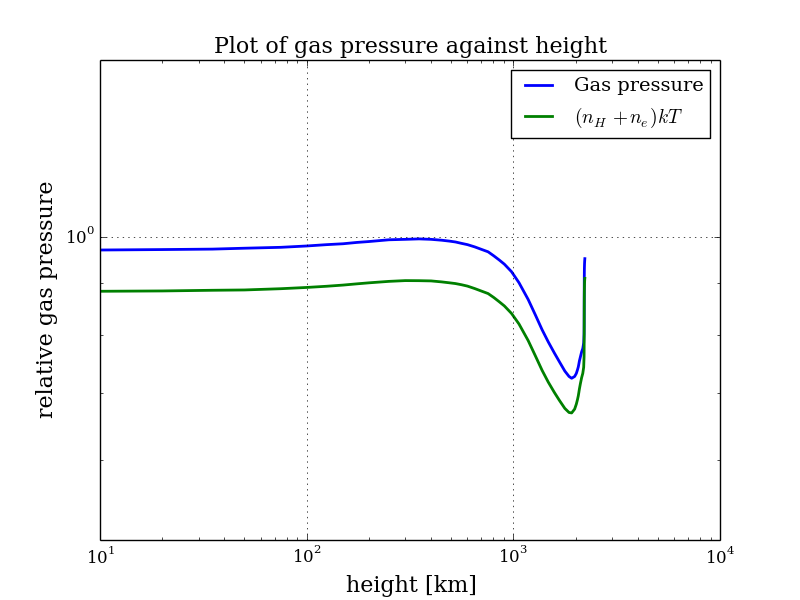
\includegraphics[scale=0.37]{../figures/falc/falc_h_pgas_1.png}
    \caption{Relative gas pressure against height, log $x$, log $y$.}
  \end{subfigure}
  \begin{subfigure}{0.49\textwidth}
    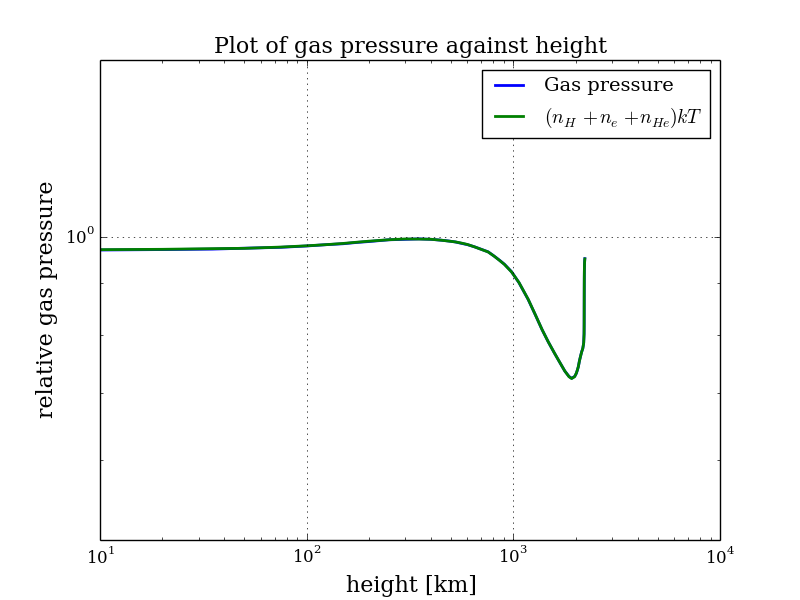
\includegraphics[scale=0.37]{../figures/falc/falc_h_pgas_2.png}
    \caption{Relative gas pressure with He added to IG, log $x$, log $y$.}
  \end{subfigure}
  \caption{Relative gas pressure ($P_{g}/P_{\text{tot}}$) against height. Overplotted is ideal gas for hydrogen and free electrons. On the panel to the right, helium is also added to the ideal gas law. We see that by adding helium, the ideal gas law overlaps the FALC data pretty much perfectly.}
\end{figure}

\subsubsection{Number densities against height}
\begin{figure}[H]
  \centering
  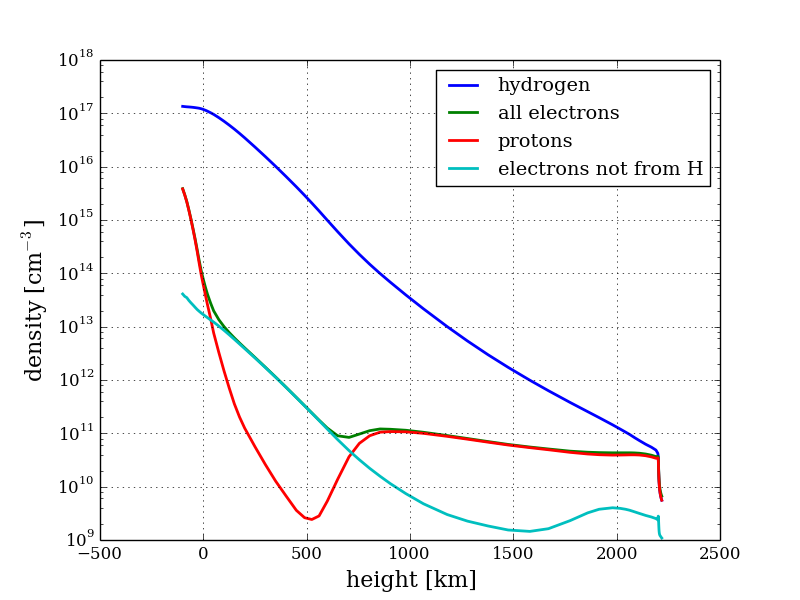
\includegraphics[scale=0.5]{../figures/falc/falc_h_n_log.png}
  \caption{Plot of number densities for the different components of the Sun, against height, plotted with logarithmic $y$-axis. We see that there is a dip the proton density at $h\approx500$ km, which we remember was the temperature minimum in our temperature stratification plot. It makes sense that the free proton density is at its lowest there, as the gas is coldest, and less hydrogen will be ionized. All number densities decrease with increasing height, as the mass density drops. The cyan curve, representing electrons not coming from hydrogen is parallel to the hydrogen density in the photosphere, and low chromosphere, where the temperature is fairly low and changes slowly. This implies that for low heights, the metal abundance compared to hydrogen is constant. As we start going towards the corona, the cyan curve has a bump as the temperature increases, and metals are ionized more, releasing more electrons.}
\end{figure}

\subsubsection{Ionization fraction of hydrogen}
\begin{figure}[H]
  \centering
  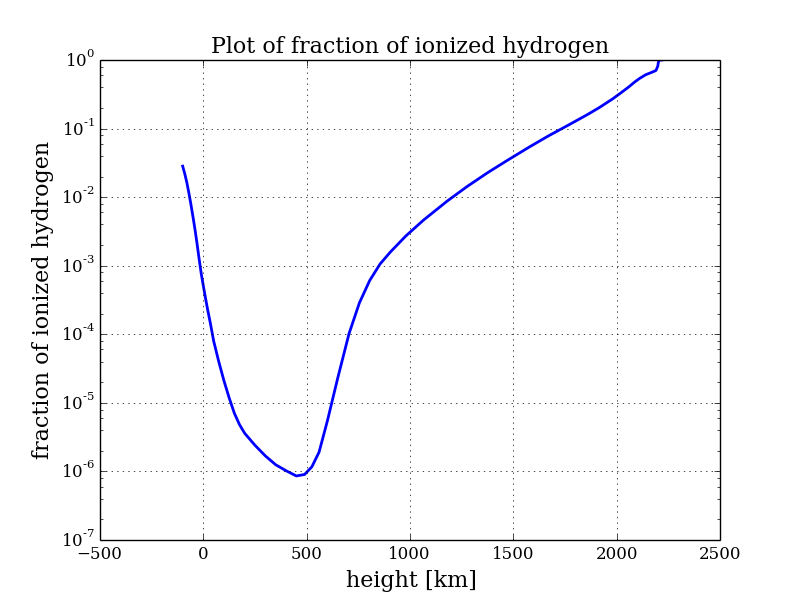
\includegraphics[scale=0.5]{../figures/falc/falc_h_Hion.png}
  \caption{Plot of the fraction of ionized hydrogen to total hydrogen, against height, with logarithmic $y$-axis. We see that it reaches a minimum around $h=500$ km, as one would expect, since that is where figure \ref{fig:falc_temp} of the temperature reaches a minimum.}
\end{figure}

\subsubsection{Photon density and particle density}
We approximate the photon density to $N_{\text{photons}} \approx 20T^3$, which holds for thermodynamic equilibrium and isotropic radiation. For lower parts of the atmosphere, these are satisfied, but higher up, the density is too low for TE, so we approximate it to $N_{\text{photons}} \approx 20T_{\text{eff}}^3/2\pi$, where $T_{\text{eff}} = 5770$ K.\\\\
At the lowest part of the atmosphere, $h = -100$ km:
\begin{align*}
  N_{\text{hydrogen}} &= 1.351\cdot10^{17} \,\text{cm}^{-3}\\
  N_{\text{photons}} &= 1.661\cdot10^{13}\,\text{cm}^{-3}\\
  \frac{N_{\text{photons}}}{N_{\text{hydrogen}}} &= 1.230\cdot10^{-4}
\end{align*}
At the highest part of the atmosphere, $h = 2218.2$ km:
\begin{align*}
  N_{\text{hydrogen}} &= 5.575\cdot10^{9} \,\text{cm}^{-3}\\
  N_{\text{photons}} &= 6.115\cdot10^{11}\,\text{cm}^{-3}\\
  \frac{N_{\text{photons}}}{N_{\text{hydrogen}}} &= 109.68
\end{align*}
We see that in the lower atmosphere, the photon density is insignificant compared to the hydrogen density, while being completely dominant in the upper part of the atmosphere. The medium there is insensitive to these photons as the density is so low that collisions are very very rare. The Ly$\alpha$ line is a resonant line for hydrogen, so the hydrogen there can absorb and emit Ly$\alpha$.

\subsection{Comparison with the Earth's atmosphere}
\subsubsection{Data from Earth's atmosphere}

\begin{figure}[H]
  \centering
  \begin{subfigure}{0.49\textwidth}
    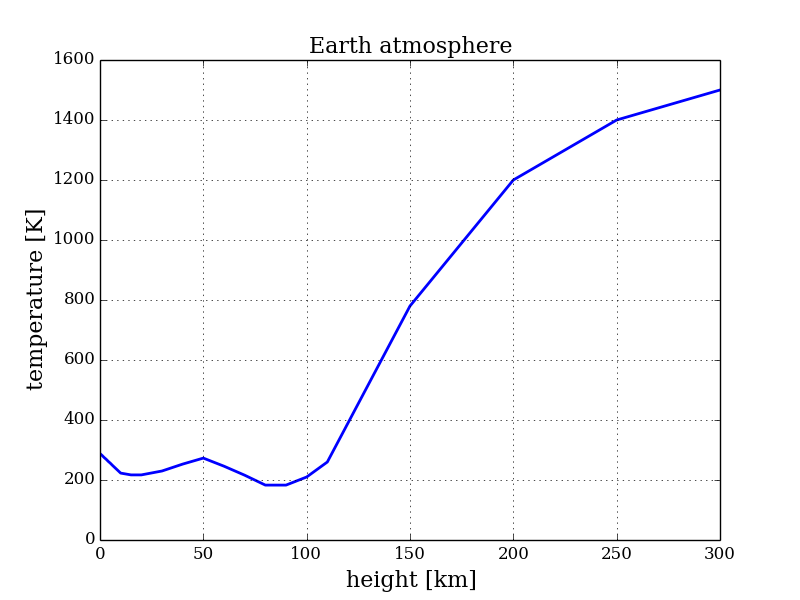
\includegraphics[scale=0.37]{../figures/earth/earth_h_temp.png}
    \caption{Temperature against height}
  \end{subfigure}
  \begin{subfigure}{0.49\textwidth}
    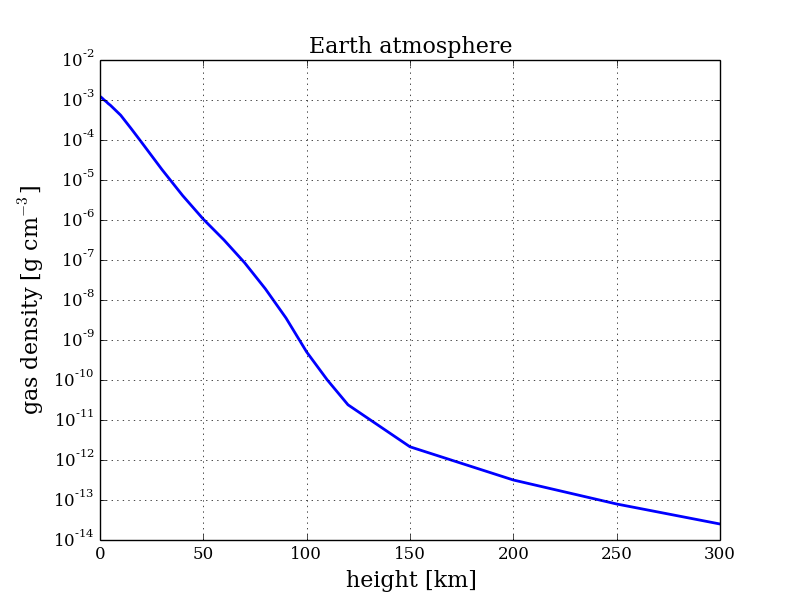
\includegraphics[scale=0.37]{../figures/earth/earth_h_rho.png}
    \caption{Gas density against height, log $y$.}
  \end{subfigure}
  \\
  \begin{subfigure}{0.49\textwidth}
    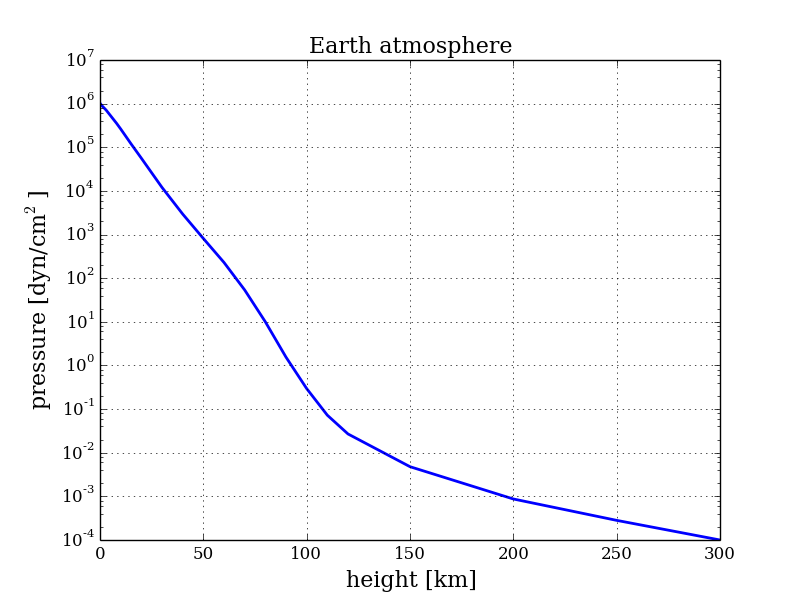
\includegraphics[scale=0.37]{../figures/earth/earth_h_P.png}
    \caption{Gas pressure against height, log $y$.}
  \end{subfigure}
  \begin{subfigure}{0.49\textwidth}
    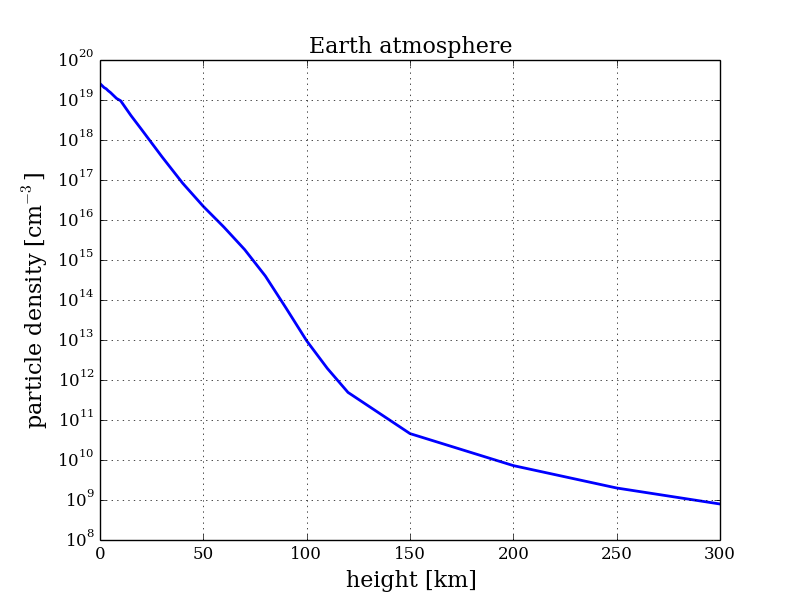
\includegraphics[scale=0.37]{../figures/earth/earth_h_N.png}
    \caption{Particle density against height, log $y$.}
  \end{subfigure}
  \caption{We see that the temperature is fairly stable until $h=120$ km, where it starts increasing for some reason. The other panels decrease with increasing height like you would expect.}
\end{figure}

\subsubsection{Normalized pressure, gas and number densities}
\begin{figure}[H]
  \centering
  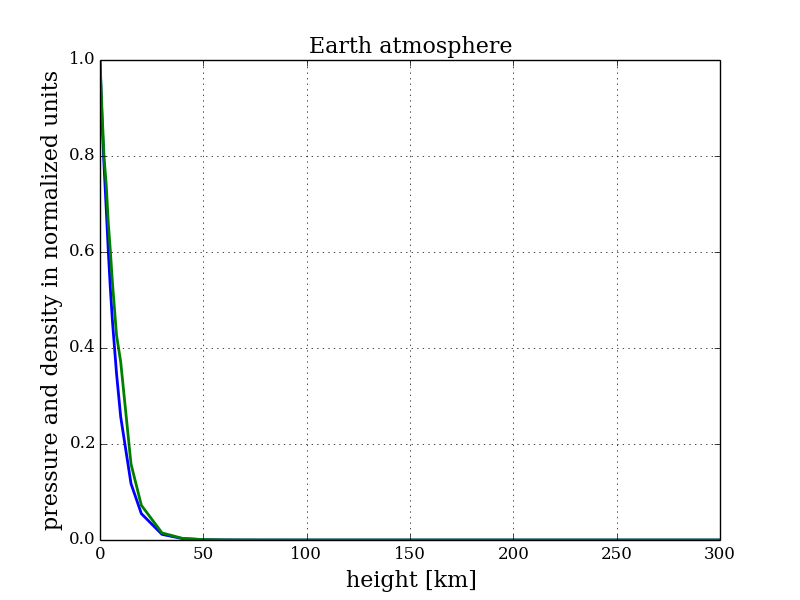
\includegraphics[scale=0.5]{../figures/earth/earth_h_PN.png}
  \caption{Plot of normalized pressure, gas and number densities against height. For lower heights, they all decrease fairly identical, but at around $h=120$ km, the slope of the logarithmic curves change. This was also the height where the temperature also started to change its behavior.}
\end{figure}

\subsubsection{Mean molecular weight}
\begin{figure}[H]
  \centering
  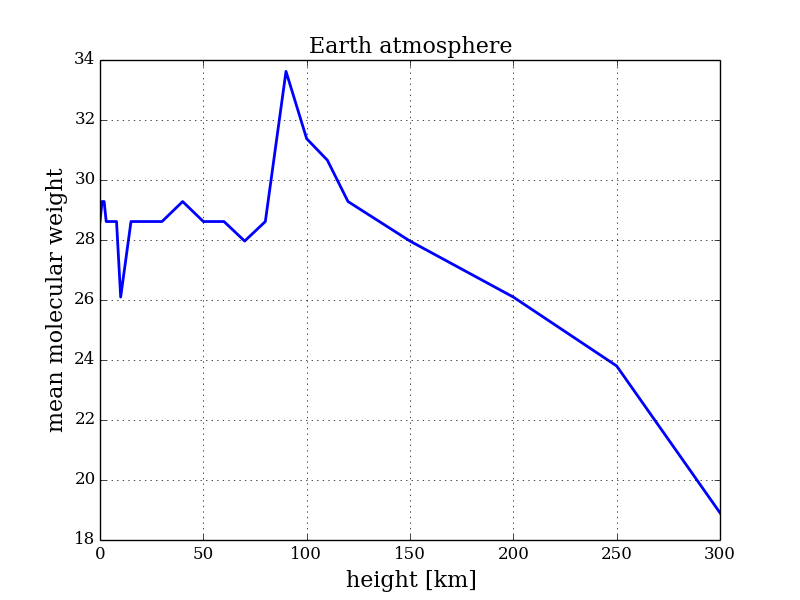
\includegraphics[scale=0.5]{../figures/earth/earth_h_mu.png}
  \caption{The mean molecular weight plotted against height. We see that for heights over $h=120$ km (the same height again), the mean molecular weight decreases with increasing height. This is due to the fact that the heavier elements will flow downwards, while lighter elements will be buoyant, and rise upwards.}
\end{figure}
\subsubsection{Calculating and comparing to the Sun}
Like we did with the Sun, we can calculate the density scale height for the lower atmosphere. This gives us $H_{\rho} = 10$ km. Using this (and the fact that Mount Everest is 8.848 km tall), we calculate that it is 42.2\% harder to breath at Mount Everest than at the surface.\\\\
We compare the density scale height with the one we found for the lower Sun surface
\begin{align*}
  \frac{N_{\text{Earth}}}{N_{\text{Sun}}} = 197.575
\end{align*}
Using that the standard gravity at the Earth's atmosphere is $g_{\text{E}} = 980.665$ cm s$^{-2}$, we estimate the atmospheric column mass to be
\begin{align*}
  m = 1043.468 \,\text{g cm$^{-2}$}
\end{align*}
The column mass at the base of the stellar photosphere was $m = 4.404$ g cm$^{-2}$, so the one on earth is considerable higher.\\\\
The sunshine photon density at earth is given by
\begin{align*}
N_{\text{phot}} = \pi\frac{R^2}{D^2}N_{\text{phot}}^{\text{top}}
\end{align*}
with $N_{\text{phot}}^{\text{top}} = 6.115\cdot10^{11}\,\text{cm}^{-3}$, $R$ the solar radius and $D$ the distance sun-earth. This gives us
\begin{align*}
  N_{\text{phot}} = 4.152\cdot10^7\,\text{cm}^{-3}
  \intertext{the particle density in the air is}
  N_{\text{part}} = 2.570\cdot10^{19}\,\text{cm}^{-3}
  \intertext{and the local thermal photon production}
  N_{\text{phot}}^{\text{loc}} = 4.778\cdot10^{8}\,\text{cm}^{-3}
\end{align*}
The local thermal photon production is higher than the one coming from the sun, so could maybe indicate that the LTE assumption does not hold that well in low Earth atmosphere.

\section{Continuous spectrum from the solar atmosphere}
\subsection{Observed solar continua}
\begin{figure}[H]
  \centering
  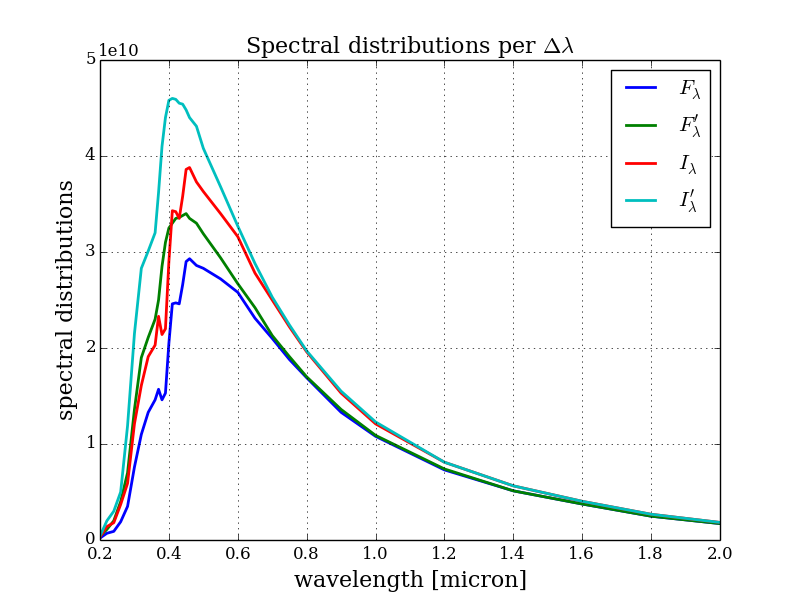
\includegraphics[scale=0.5]{../figures/task2/solspect_lambda_spec_dist.png}
  \caption{Plot of the four spectral distributions against wavelength. They have the same unit as intensity is a measure of flux per solid angle.}
\end{figure}

\begin{figure}[H]
  \centering
  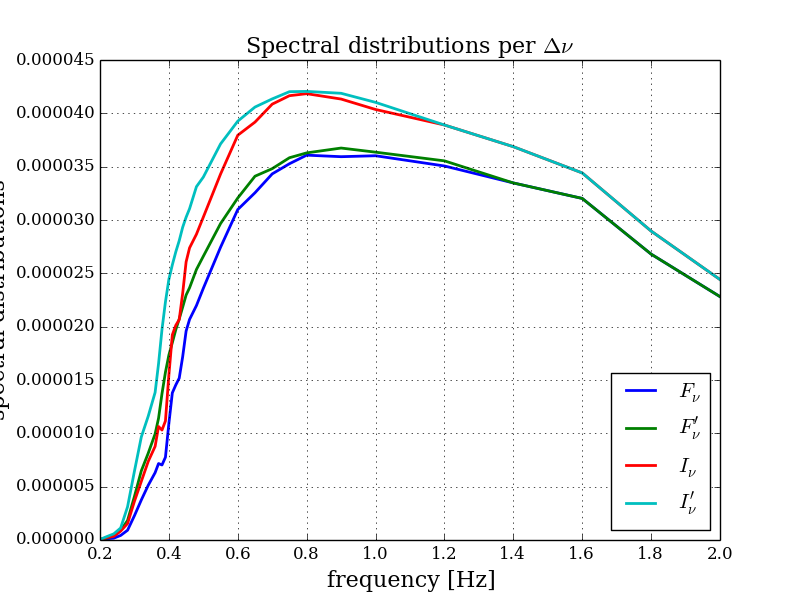
\includegraphics[scale=0.5]{../figures/task2/solspect_lambda_spec_dist_nu.png}
  \caption{Plot of the four spectral distributions per frequency bandwidth $\Delta \nu = 1$ Hz.}
\end{figure}

\begin{figure}[H]
  \centering
  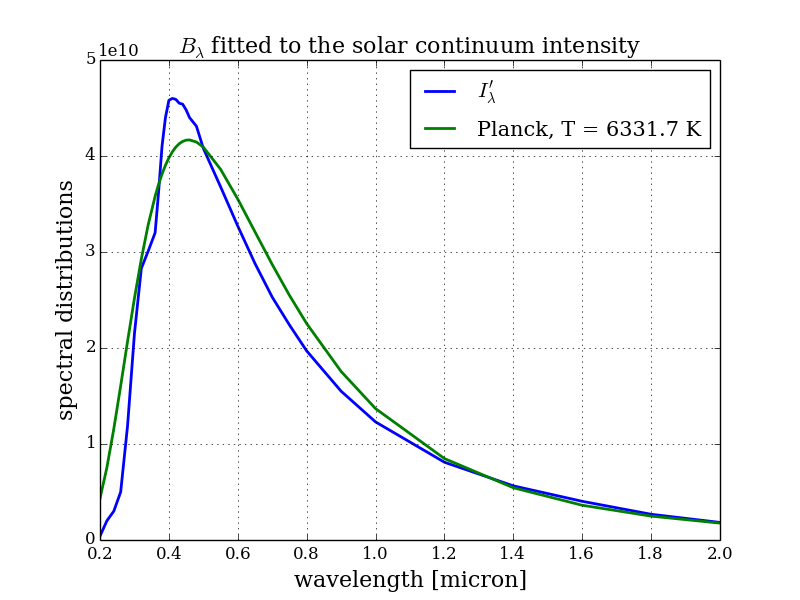
\includegraphics[scale=0.5]{../figures/task2/solspect_h_planck.png}
  \caption{Plot of continuum intensity with a Planck function fitted to it. The Planck function gives us the best fit for temperature $T = 6331.7$ K.} 
\end{figure}

\begin{figure}[H]
  \centering
  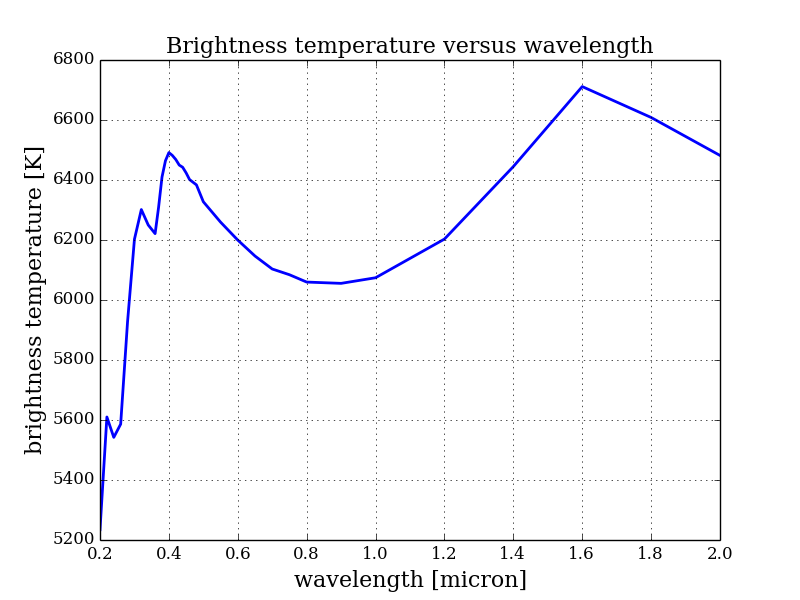
\includegraphics[scale=0.5]{../figures/task2/solspect_h_Tb.png}
  \caption{Plot of the inverted Planck function versus wavelength. This gives us the brightness temperature $T_b$ for a wavelength. The shape of this curve looks a lot like an inverse version of figure 5 from the assignment. It peaks at around $\lambda = 1.6\,\mu$m, which means that the Sun should be fairly transparent to this wavelength, and that most of the radiation escapes, resulting in a high brightness temperature.}
\end{figure}

\subsection{Continuous extinction}
\begin{figure}[H]
  \centering
  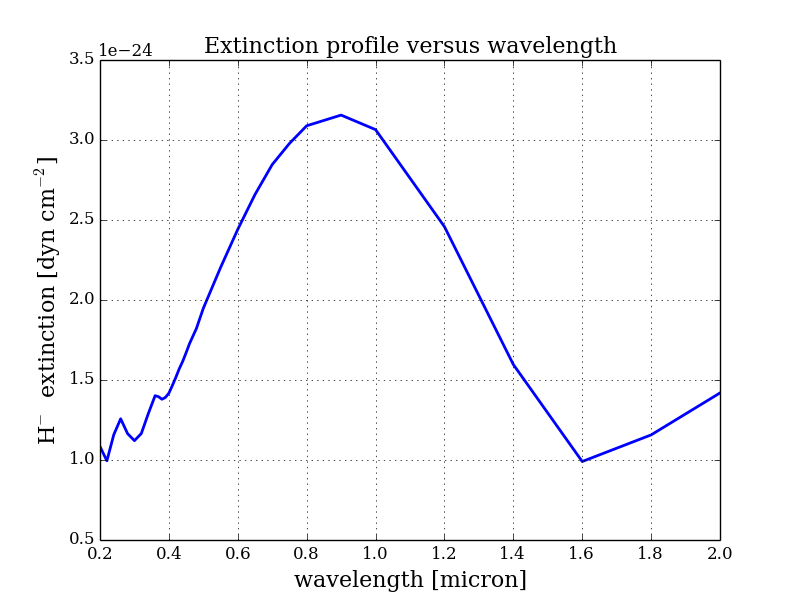
\includegraphics[scale=0.5]{../figures/task2/exthmin_lam_kappa.png}
  \caption{Extinction coefficient plotted against wavelength. We see that this looks quite a lot like Gray's version (figure 5 in SSB). However after the peak, it does not just decay over $\simeq \lambda^3$, as is more close to the total extinction rather than just from H$_{\text{bf}}^-$. We see that this is close to the solar brightness temperature plot with wavelength, or more strictly inverse of each other.}
\end{figure}

\begin{figure}[H]
  \centering
  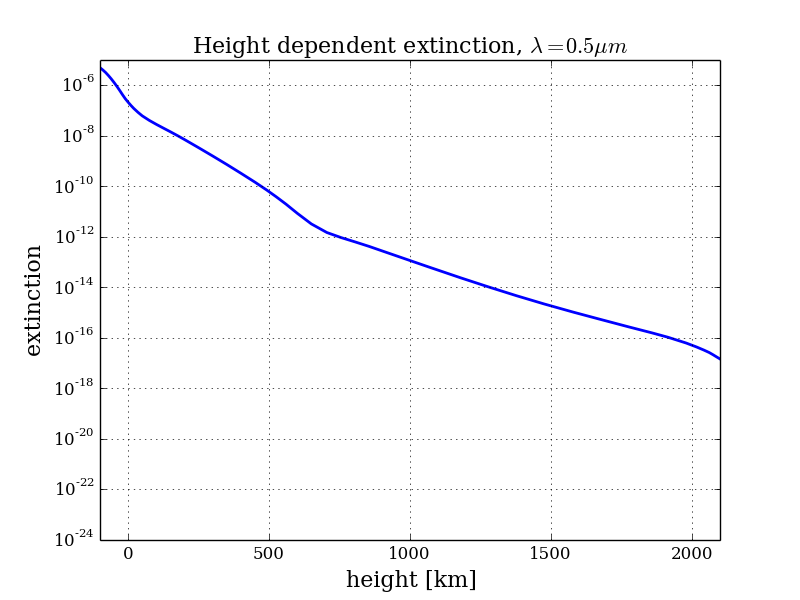
\includegraphics[scale=0.5]{../figures/task2/exthmin_2.png}
  \caption{H${^-}$ extinction per cm with height for $\lambda = 0.5\,\mu$m, log $y$.}
\end{figure}

\begin{figure}[H]
  \centering
  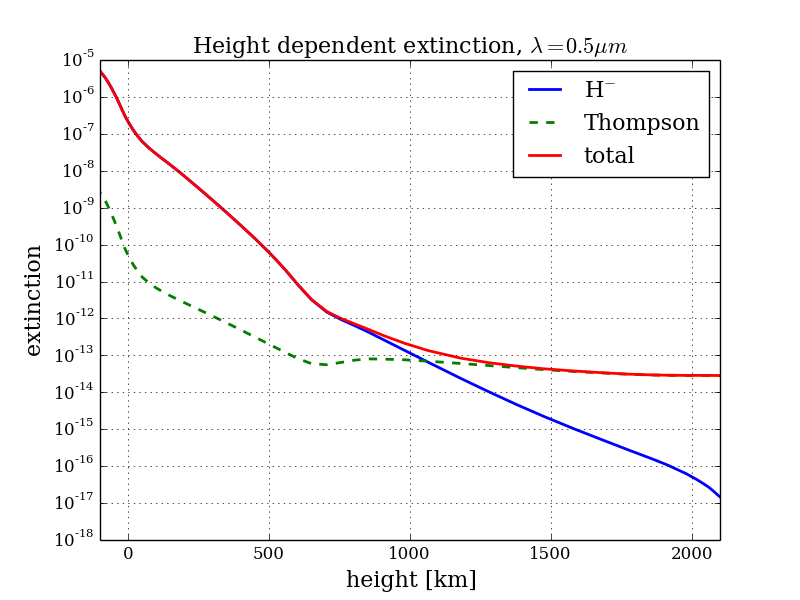
\includegraphics[scale=0.5]{../figures/task2/exthmin_3.png}
  \caption{Extinction per cm with height for $\lambda = 0.5\,\mu$m, log $y$. Unlike the last figure, H$^-$ extinction is now measured per neutral hydrogen atom. Thompson scattering off free electrons is also added to the extinction per cm by the constant $\sigma^{\text{T}} = 6.648\times10^{-25}$ cm$^2$, and multiplying with the electron number density to get correct units. Also plotted, is the total continuous extinction.\\\\For low heights, we see that the $H^{-}$ extinction dominates, and for higher heights, the Thompson scattering dominates. This follows from how the ionization fraction of hydrogen increases after it reaches the minimum at $h\approx500$ km, and the number density of neutral hydrogen decreases.}
\end{figure}

\subsection{Optical depth}
\begin{figure}[H]
  \centering
  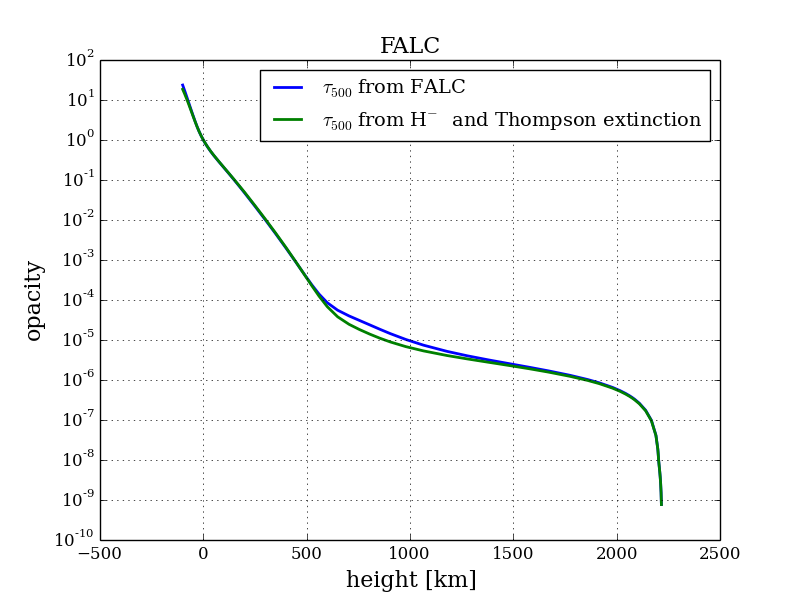
\includegraphics[scale=0.5]{../figures/task2/exthmin_h_tau.png}
  \caption{Integrated extinction at $\lambda=500$ nm to get the optical depth scale $\tau_{\lambda}(h_0)$, plotted against height. Overplotted is the FALC $\tau_{500}$ scale. We see that our code reproduces the $\tau_{500}$ results very well for low and high heights, but not so well in between.}
\end{figure}

\subsection{Emergent intensity and height of formation}
We can now compute the intensity of the radiation that emerges from the center of the solar disk, by integration as explained in the exercise text. Doing this for $\lambda = 500$ nm, gives us the following computed intensity, which we can compare to the continuum intensity we looked at earlier.
\begin{align*}
  I_{\text{computed}} &= 4.26826\cdot10^{14} \text{erg}\text{s}^{-1}\text{cm}^{-2}\text{ster}^{-1}\\
  I_{\text{observed}} &= 4.08\cdot10^{14} \text{erg}\text{s}^{-1}\text{cm}^{-2}\text{ster}^{-1}
\end{align*}
\begin{figure}[H]
  \centering
  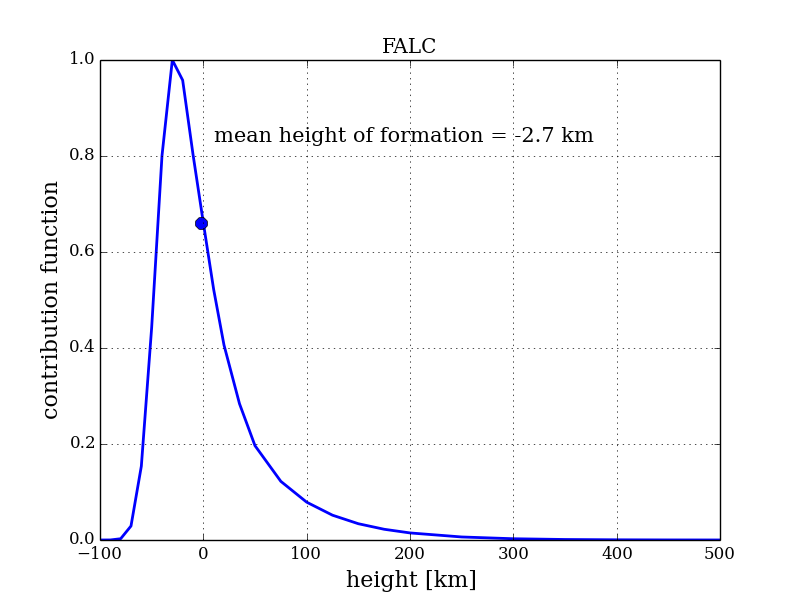
\includegraphics[scale=0.5]{../figures/task2/emergent_intensity_1.png}
  \caption{Peak-normalized contribution function plotted against height. Overplotted as a point is the mean height of formation. For $\lambda=500$ nm.}
\end{figure}

\begin{figure}[H]
  \centering
  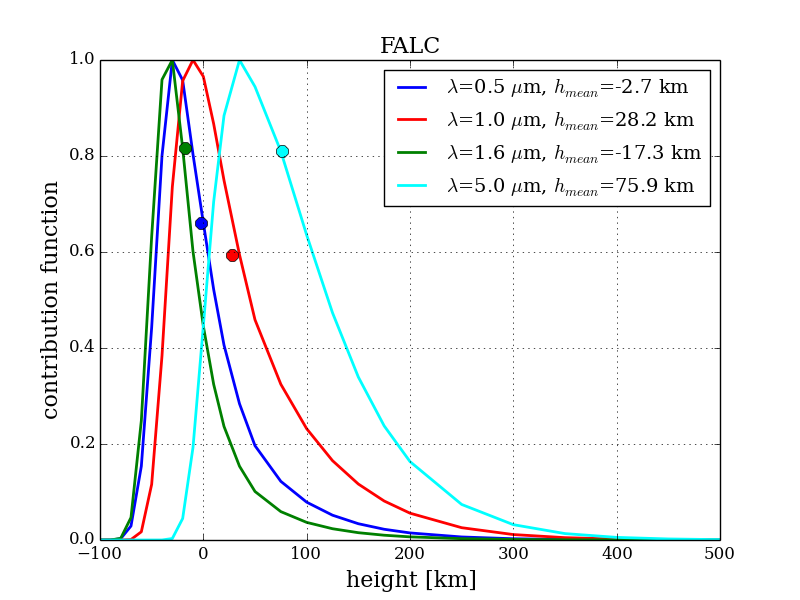
\includegraphics[scale=0.5]{../figures/task2/emergent_intensity_2.png}
  \caption{Peak-normalized contribution function plotted against height for different wavelengths $\lambda$. Overplotted as a point is the mean height of formation.}
\end{figure}

\subsection{Disk-center intensity}
\begin{figure}[H]
  \centering
  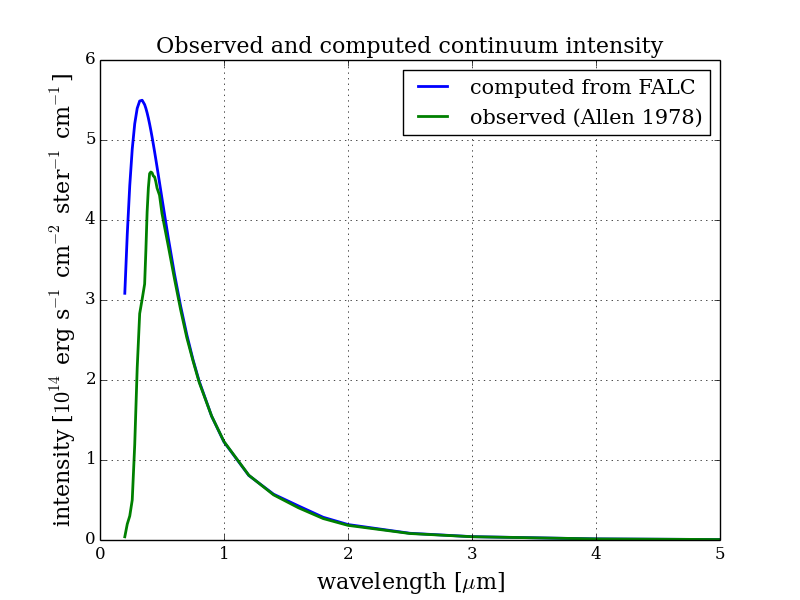
\includegraphics[scale=0.5]{../figures/task2/disc_center.png}
  \caption{Disk-center intensity plotted against wavelength. Overplotted is the observed solar continuum in \texttt{solspect.dat}.}
\end{figure}

\subsection{Limb darkening}
We can modify out code for disk-center intensity to give the intensity that emerges under an angle $\mu = \cos\theta$.
\begin{figure}[H]
  \centering
  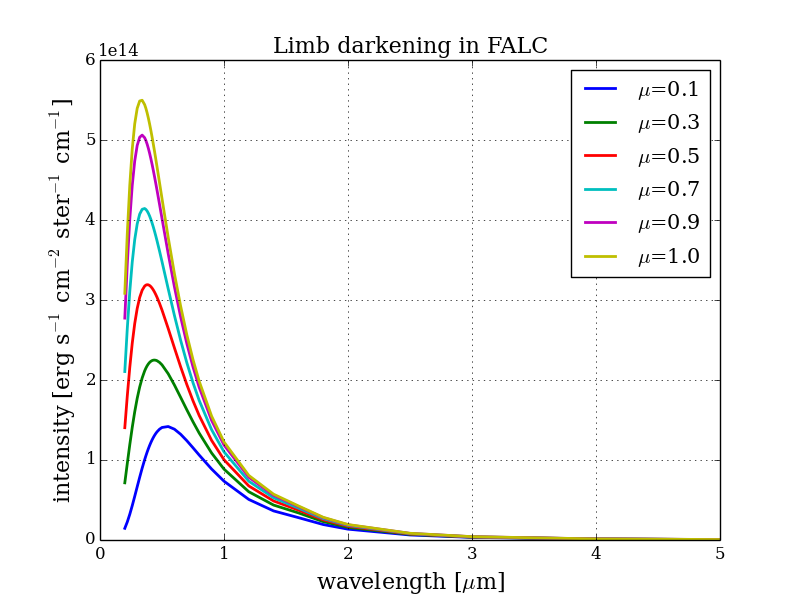
\includegraphics[scale=0.5]{../figures/task2/limb_darkening_1.png}
  \caption{Intensity evaluated for multiple values of $\mu$, plotted against wavelength. We see that for lower values of $\mu$, the intensity peaks drop down quite a lot.}
\end{figure}
Was not successfull in creating the plots for the next part of this subsection, and thus there are no more plots here.

\subsection{Flux integration}
\begin{figure}[H]
  \centering
  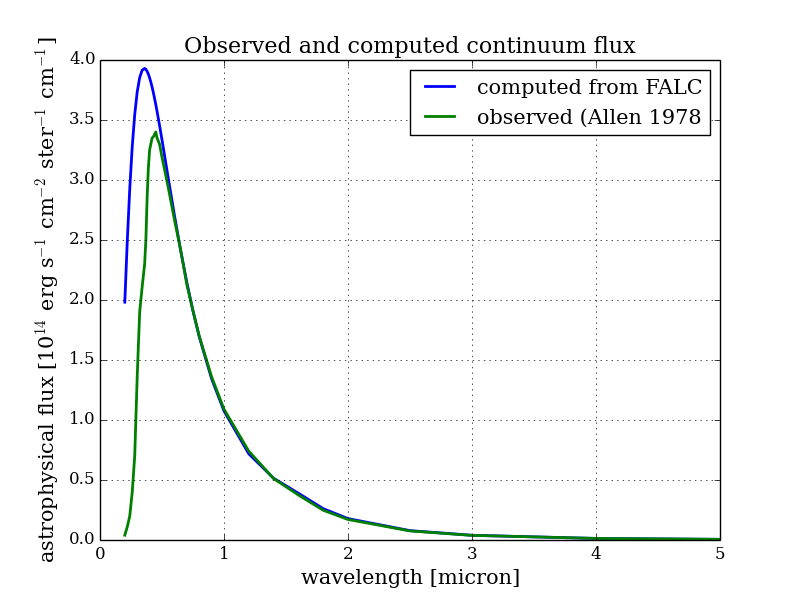
\includegraphics[scale=0.5]{../figures/task2/flux.png}
  \caption{Emergent solar flux plotted against wavelength. Overplotted is the measured flux from \texttt{solspect.dat}. We see that the figure is very similar to the one for the emergent intensity, which is maybe not very surprising given how similar in shape the four spectral distributions we plotted earlier were.}
\end{figure}

\section{Spectral lines from the solar atmosphere}
\subsection{Observed Na D line profiles and Na D wavelengths}
We start by reading in the data from the data file
\begin{figure}[H]
  \centering
  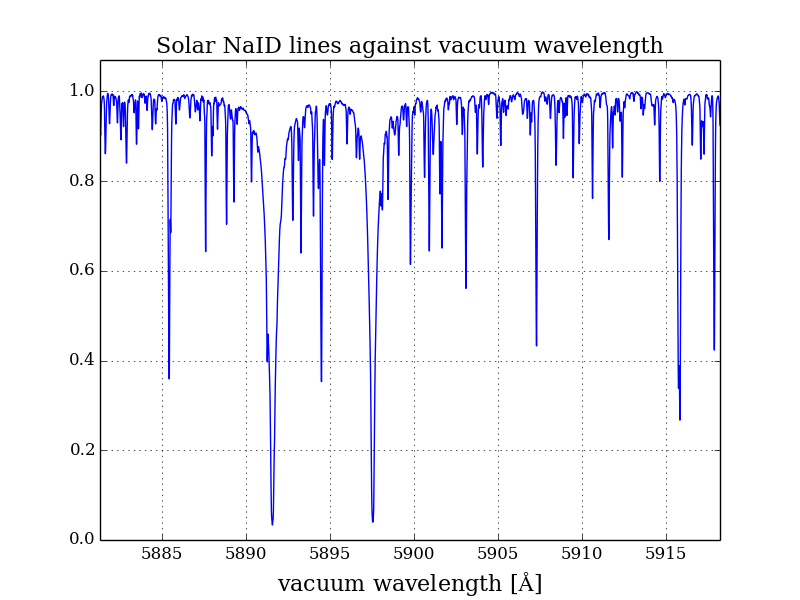
\includegraphics[scale=0.5]{../figures/task3/NaID_wav_vac_sigma.png}
  \caption{Solar disk-center intensity plotted against vacuum wavelengths. We find the location of the minimas to be in $\lambda_1 = 5891.58$ Å, and $\lambda_2 = 5897.55$ Å.}
\end{figure}
\begin{figure}[H]
  \centering
  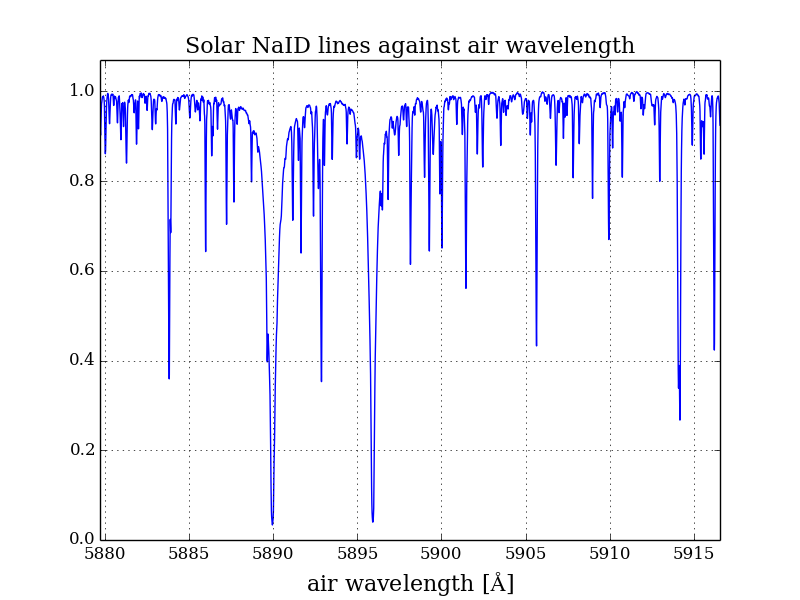
\includegraphics[scale=0.5]{../figures/task3/NaID_wav_air_sigma.png}
  \caption{Solar disk-center intensity plotted against air wavelengths. We find the location of the minimas to be in $\lambda_1 = 5889.95$ Å, and $\lambda_2 = 5895.92$ Å. We observe that the minimas are very close to the expected location of the lines.}
\end{figure}

\subsection{Implementing LTE line formation}
We test to see if our implementation of the Saha-Boltzmann distributions return reasonable results.
\begin{figure}[H]
  \centering
  \begin{subfigure}{0.49\textwidth}
    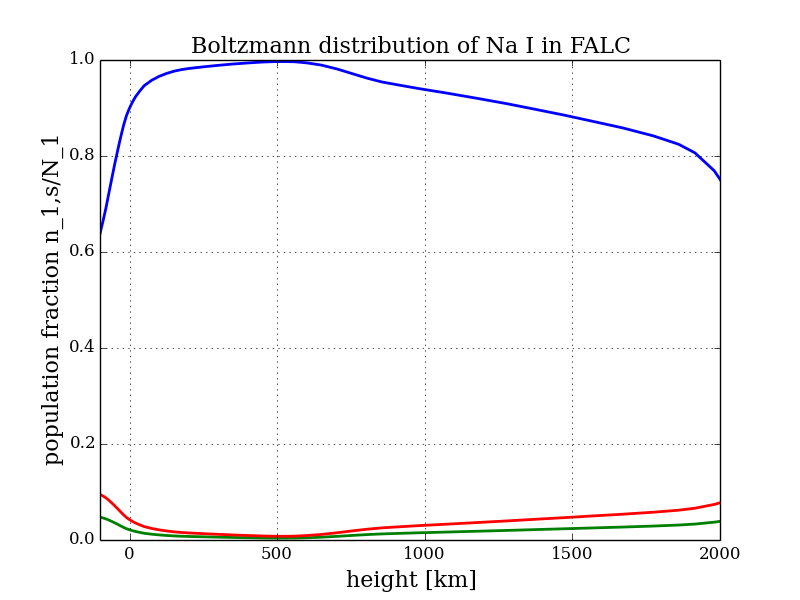
\includegraphics[scale=0.37]{../figures/task3/boltzmann.png}
    \caption{Boltzmann distribution for different excitation levels $s$.}
  \end{subfigure}
  \begin{subfigure}{0.49\textwidth}
    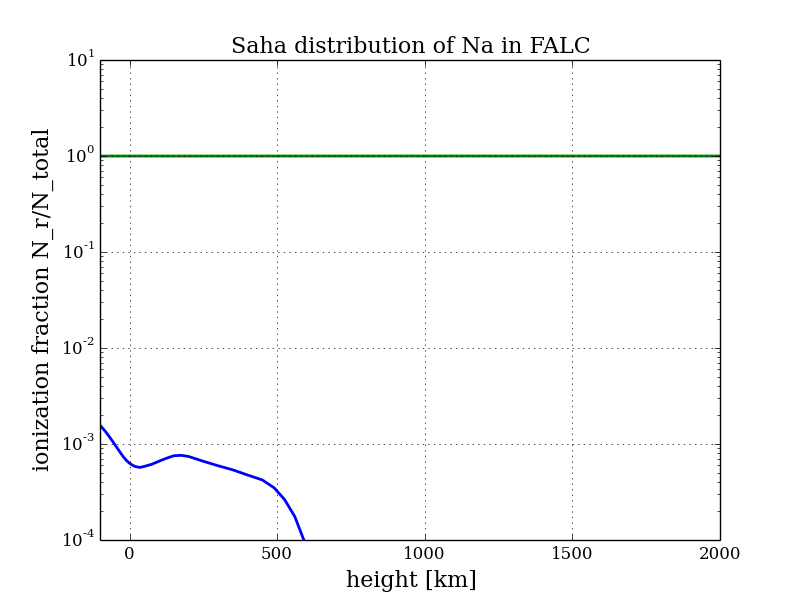
\includegraphics[scale=0.37]{../figures/task3/saha.png}
    \caption{Saha distribution for different ionization levels $r$.}
  \end{subfigure}
  \caption{The panels show that the Saha-Boltzmann functions for Na gives the results we would expect, based on the figure shown to us.}
\end{figure}

\subsection{Computed Na D$_1$ line profile}

\begin{figure}[H]
  \centering
  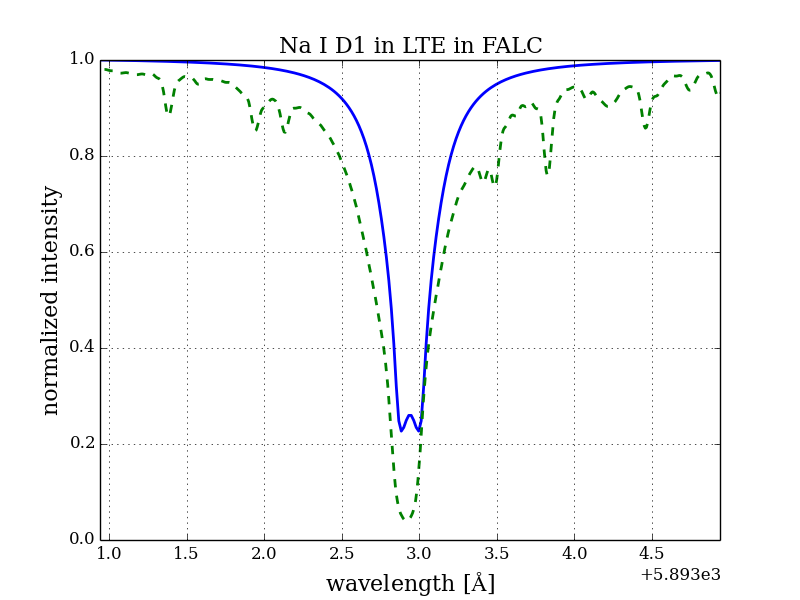
\includegraphics[scale=0.5]{../figures/Na_D1.png}
  \caption{The final computed Na D$_1$ line profile plotted against wavelength. Overplotted in dashed lines is the observed Na D line profile we plotted earlier. We see that the computed line follows roughly the same shape as the observed line profile. One of the differences, is that our line does not go as deep, and that at the center, line-center reversal occurs. Our model is a fairly decent model for photospheric lines, but one of the key assumptions of our model was LTE. Since the computed line profile reproduces the core poorly, we can assume that the assumption of LTE breaks down for the core.}
\end{figure}

Following tradition, we add a collisional enhancement factor $E$ to the $\gamma_{\text{vdW}}$, in order to attempt obtaining a better fit of the line wings.
\begin{figure}[H]
  \centering
  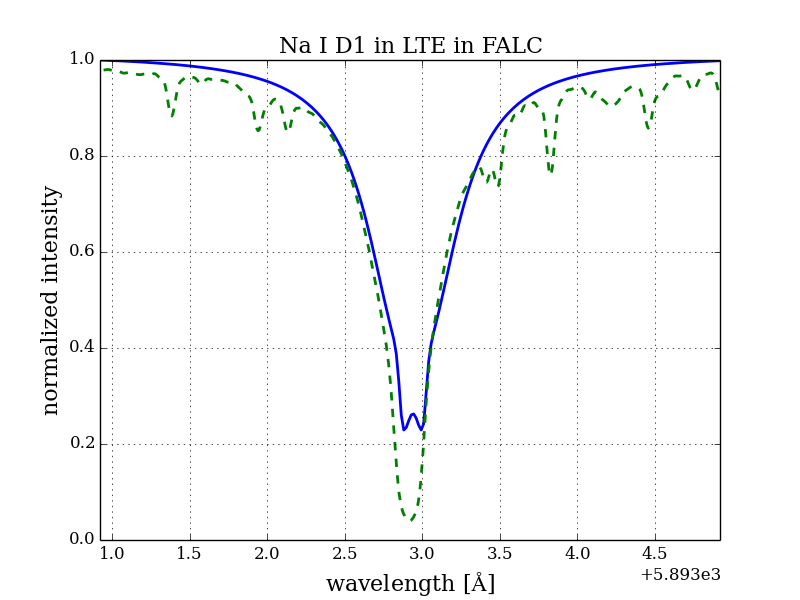
\includegraphics[scale=0.5]{../figures/task3/Na_D1.png}
  \caption{Computed line profile plotted against wavelength, with the observed line profile overplotted. Here we have after experimenting set the fudge factor $E$ to $E=3$ in order to get a better fit. As we see, it fits the observed data better than without the factor.}
\end{figure}
\section{Appendix - Python code}
All code used can be found in the GitHub repository located at\\\href{https://github.com/simennb/ast4310/tree/master/exercise2/src}{https://github.com/simennb/ast4310/tree/master/exercise2/src}
\\The python-code is also appended below
\subsection{General tools and functions for all programs}
\verbatiminput{../src/ssb.py}
\subsection{FALC plotting}
\verbatiminput{../src/falc.py}
\subsection{Earth plotting}
\verbatiminput{../src/earth.py}
\subsection{Exercise 2.1}
\verbatiminput{../src/task2.py}
\subsection{Rest of exercise 2}
\verbatiminput{../src/task2_2.py}
\subsection{Exercise 3}
\verbatiminput{../src/task3.py}

\end{document}
